\documentclass[tikz,border=8pt]{standalone}

\usepackage[T1]{fontenc}
\usepackage{helvet}
\usepackage{xcolor}
\usetikzlibrary{arrows.meta,backgrounds,calc,fit,matrix,positioning,shapes.geometric}

% Muted categorical colors keep block types readable without the brighter
% pastel treatment; typography and square outlines carry the schematic style.
\definecolor{bjFunctionalFill}{HTML}{DFEAF3}
\definecolor{bjFunctionalEdge}{HTML}{3F6D91}
\definecolor{bjBufferFill}{HTML}{E1EEE6}
\definecolor{bjBufferEdge}{HTML}{477968}
\definecolor{bjTableFill}{HTML}{F6ECD9}
\definecolor{bjTableEdge}{HTML}{9A7638}
\definecolor{bjControlFill}{HTML}{E9E6F2}
\definecolor{bjControlEdge}{HTML}{69618A}
\definecolor{bjExternalFill}{HTML}{FFFFFF}
\definecolor{bjExternalEdge}{HTML}{41474C}
\definecolor{bjRegionFill}{HTML}{FFFFFF}
\definecolor{bjRegionEdge}{HTML}{737A80}
\definecolor{bjData}{HTML}{29333B}
\definecolor{bjControl}{HTML}{69618A}
\definecolor{bjLookup}{HTML}{9A7638}
\definecolor{bjClock}{HTML}{A45140}

\tikzset{
  font=\sffamily,
  major/.style={
    rectangle, draw=bjFunctionalEdge,
    fill=bjFunctionalFill, line width=0.9pt, align=center,
    minimum height=12mm, minimum width=25mm, inner sep=4pt
  },
  mux/.style={
    trapezium, trapezium stretches=true,
    trapezium left angle=70, trapezium right angle=70,
    shape border rotate=270, draw=bjFunctionalEdge,
    fill=bjFunctionalFill, line width=0.9pt, align=center,
    minimum width=38mm, minimum height=18mm, inner sep=4pt
  },
  fifo/.style={
    rectangle, draw=bjBufferEdge, fill=bjBufferFill,
    line width=0.9pt, align=center, minimum height=10mm,
    minimum width=18mm, inner sep=3pt
  },
  rom/.style={
    rectangle, draw=bjTableEdge, fill=bjTableFill,
    line width=0.9pt, align=center, minimum height=12mm,
    minimum width=30mm, inner sep=4pt
  },
  controlblock/.style={
    rectangle, draw=bjControlEdge,
    fill=bjControlFill, line width=0.9pt, align=center,
    minimum height=12mm, minimum width=30mm, inner sep=4pt
  },
  csrrow/.style={
    rectangle, draw=bjControlEdge, fill=bjControlFill!45!white,
    line width=0.65pt, align=center, font=\sffamily\scriptsize,
    minimum height=5.8mm, minimum width=32mm, inner sep=1.5pt
  },
  external/.style={
    rectangle, draw=bjExternalEdge, fill=bjExternalFill,
    line width=1.0pt, align=center, minimum height=12mm,
    minimum width=22mm, inner sep=4pt
  },
  subsystem/.style={
    rectangle, draw=bjRegionEdge,
    fill=bjRegionFill, fill opacity=0.34, text opacity=1,
    dashed, line width=0.9pt, inner sep=7pt
  },
  datapath/.style={
    -{Stealth[length=2.6mm,width=1.9mm]}, draw=bjData,
    line width=1.4pt, line cap=rect, line join=miter
  },
  controlconn/.style={
    -{Diamond[open,length=2.4mm,width=2.1mm]}, draw=bjControl,
    draw opacity=0.9, densely dashed, line width=0.8pt,
    line cap=rect, line join=round
  },
  controlbidir/.style={
    {Diamond[open,length=2.4mm,width=2.1mm]}-{Diamond[open,length=2.4mm,width=2.1mm]},
    draw=bjControl, draw opacity=0.9, densely dashed, line width=0.8pt,
    line cap=rect, line join=round
  },
  configspine/.style={
    draw=bjControl, draw opacity=0.9, densely dashed, line width=0.95pt,
    line cap=rect, line join=round
  },
  sequencespine/.style={
    draw=bjControl, draw opacity=0.9, densely dashed, line width=0.95pt,
    line cap=rect, line join=round
  },
  lookupconn/.style={
    {Stealth[length=2.4mm,width=1.8mm]}-{Stealth[length=2.4mm,width=1.8mm]},
    draw=bjLookup, densely dotted, line width=1.15pt,
    line cap=rect, line join=round
  },
  clockconn/.style={
    -{Stealth[length=2.6mm,width=2.0mm]},
    draw=bjClock, dash pattern=on 5pt off 2pt on 1pt off 2pt,
    draw opacity=0.9, line width=0.8pt, line cap=rect, line join=round
  },
  moduleboundary/.style={
    rectangle, draw=bjData, line width=1.35pt, line cap=rect,
    line join=round
  },
  signal/.style={font=\sffamily\scriptsize, fill=none, inner sep=2pt, align=center},
  portlabel/.style={font=\sffamily\tiny, text=bjExternalEdge, inner sep=1pt},
  moduleLabel/.style={font=\sffamily\bfseries\large, text=bjRegionEdge, fill=white, inner sep=2pt},
  regionlabel/.style={font=\sffamily\bfseries\small, text=bjRegionEdge, fill=white, inner sep=2pt},
  title/.style={font=\sffamily\bfseries\Large, text=bjData},
  subtitle/.style={font=\sffamily\small, text=bjExternalEdge}
}

\begin{document}
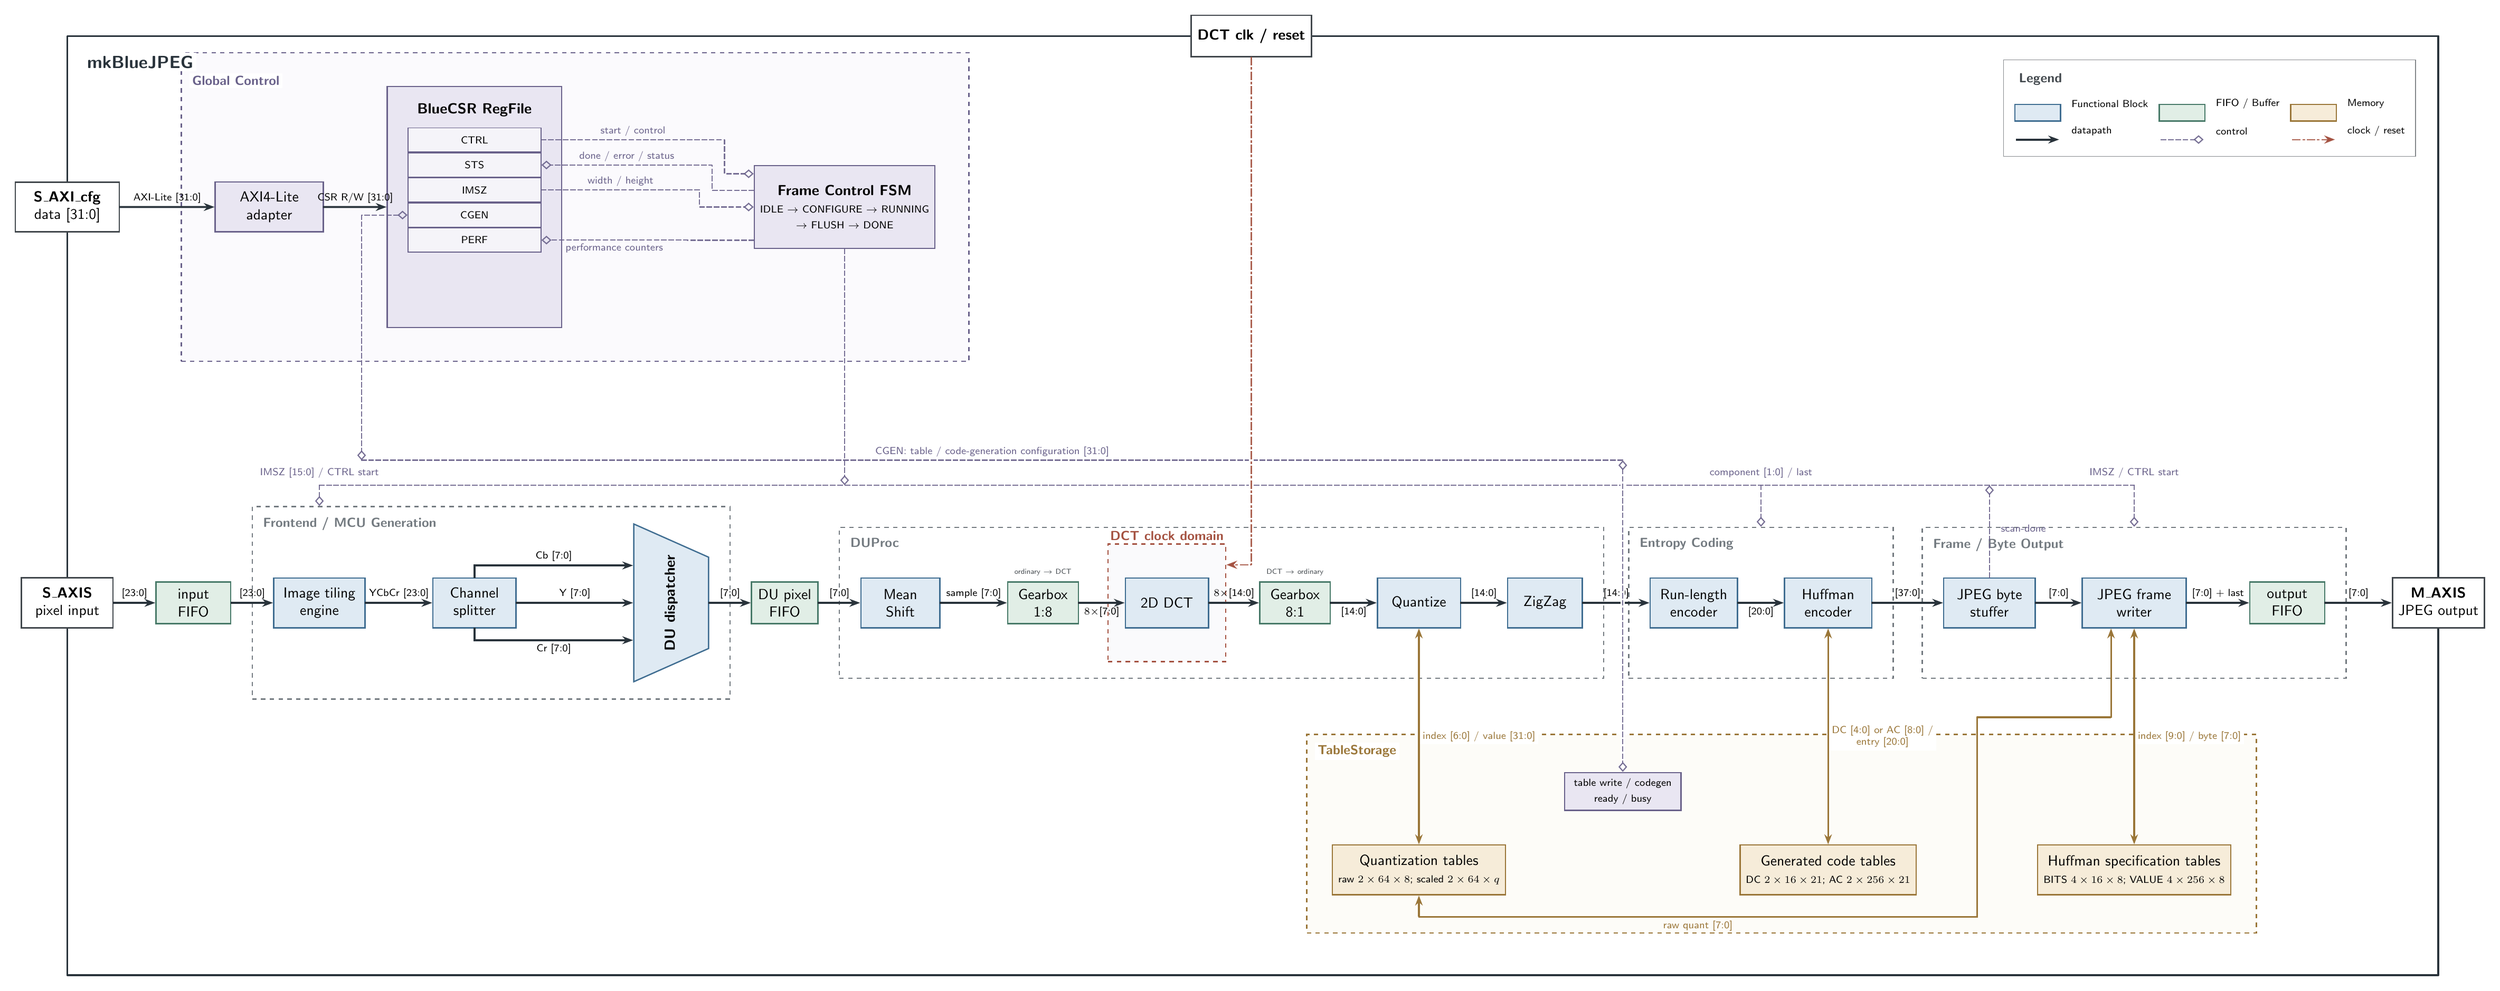
\begin{tikzpicture}[node distance=7mm and 7mm]

% ----------------------------------------------------------------------------
% Main datapath - a single, centered left-to-right reading line.
% ----------------------------------------------------------------------------
\node[external] (saxis) {\textbf{S\_AXIS}\\pixel input};
\node[fifo, right=10mm of saxis] (axisrd) {input\\FIFO};

\node[major, minimum width=22mm, right=10mm of axisrd] (tiler) {Image tiling\\engine};
\node[major, minimum width=20mm, right=16mm of tiler] (splitter) {Channel\\splitter};
\node[mux, right=28mm of splitter] (dispatcher) {};
\node[font=\sffamily\bfseries, rotate=90] at (dispatcher.center)
  {DU dispatcher};
\node[fifo, minimum width=16mm, right=10mm of dispatcher] (dufifo) {DU pixel\\FIFO};

\node[major, minimum width=19mm, right=10mm of dufifo] (meanshift) {Mean\\Shift};
\node[fifo, minimum width=17mm, right=16mm of meanshift] (gear1) {Gearbox\\1:8};
\node[major, minimum width=20mm, right=11mm of gear1] (dct) {2D DCT};
\node[fifo, minimum width=17mm, right=12mm of dct] (gear8) {Gearbox\\8:1};
\node[major, minimum width=20mm, right=11mm of gear8] (quant) {Quantize};
\node[major, minimum width=18mm, right=11mm of quant] (zigzag) {ZigZag};

\node[major, minimum width=21mm, right=16mm of zigzag] (rle) {Run-length\\encoder};
\node[major, minimum width=21mm, right=11mm of rle] (huff) {Huffman\\encoder};

\node[major, minimum width=22mm, right=17mm of huff] (stuffer) {JPEG byte\\stuffer};
\node[major, minimum width=25mm, right=11mm of stuffer] (fwriter) {JPEG frame\\writer};
\node[fifo, minimum width=18mm, right=15mm of fwriter] (axiswr) {output\\FIFO};
\node[external, right=16mm of axiswr] (maxis) {\textbf{M\_AXIS}\\JPEG output};

% Primary data connections. Labels are deliberately compact.
\draw[datapath] (saxis.east) -- node[signal, above] {[23:0]} (axisrd.west);
\draw[datapath] (axisrd.east) -- node[signal, above] {[23:0]} (tiler.west);
\draw[datapath] (tiler.east) -- node[signal, above] {YCbCr [23:0]} (splitter.west);
\draw[datapath] (splitter.east) -- node[signal, above] {Y [7:0]} (dispatcher.west);
\coordinate (cbdispatchin) at ($(dispatcher.west)+(0,9mm)$);
\coordinate (crdispatchin) at ($(dispatcher.west)+(0,-9mm)$);
\draw[datapath] (splitter.north) |- node[signal, above, near end] {Cb [7:0]} (cbdispatchin);
\draw[datapath] (splitter.south) |- node[signal, below, near end] {Cr [7:0]} (crdispatchin);
\draw[datapath] (dispatcher.east) -- node[signal, above] {[7:0]} (dufifo.west);

\draw[datapath] (dufifo.east) -- node[signal, above] {[7:0]} (meanshift.west);
\draw[datapath] (meanshift.east) -- node[signal, above] {sample [7:0]} (gear1.west);
\draw[datapath] (gear1.east) -- node[signal, below] {$8\times$[7:0]} (dct.west);
\draw[datapath] (dct.east) -- node[signal, above] {$8\times$[14:0]} (gear8.west);
\draw[datapath] (gear8.east) -- node[signal, below] {[14:0]} (quant.west);
\draw[datapath] (quant.east) -- node[signal, above] {[14:0]} (zigzag.west);
\draw[datapath] (zigzag.east) -- node[signal, above] {[14:0]} (rle.west);
\draw[datapath] (rle.east) -- node[signal, below] {[20:0]} (huff.west);
\draw[datapath] (huff.east) -- node[signal, above] {[37:0]} (stuffer.west);
\draw[datapath] (stuffer.east) -- node[signal, above] {[7:0]} (fwriter.west);
\draw[datapath] (fwriter.east) -- node[signal, above] {[7:0] + last} (axiswr.west);
\draw[datapath] (axiswr.east) -- node[signal, above] {[7:0]} (maxis.west);

% ----------------------------------------------------------------------------
% Spatial grouping: front end, DUProc, entropy coding, and frame output.
% ----------------------------------------------------------------------------
\begin{scope}[on background layer]
  \node[subsystem, fit=(tiler)(splitter)(dispatcher), inner xsep=5mm, inner ysep=8mm]
        (frontend) {};
  \node[subsystem, fit=(meanshift)(gear1)(dct)(gear8)(quant)(zigzag),
        inner xsep=5mm, inner ysep=12mm] (duproc) {};
  \node[subsystem, draw=bjClock, fill=bjControlFill, fill opacity=0.20,
        fit=(dct), inner xsep=4mm, inner ysep=8mm] (dctdomain) {};
  \node[subsystem, fit=(rle)(huff), inner xsep=5mm, inner ysep=12mm]
        (entropy) {};
  \node[subsystem, fit=(stuffer)(fwriter)(axiswr), inner xsep=5mm, inner ysep=12mm]
        (frameout) {};
\end{scope}

\node[regionlabel, anchor=north west] at ($(frontend.north west)+(2mm,-2mm)$)
  {Frontend / MCU Generation};
\node[regionlabel, anchor=north west] at ($(duproc.north west)+(2mm,-2mm)$)
  {DUProc};
\node[regionlabel, anchor=north west] at ($(entropy.north west)+(2mm,-2mm)$)
  {Entropy Coding};
\node[regionlabel, anchor=north west] at ($(frameout.north west)+(2mm,-2mm)$)
  {Frame / Byte Output};
\node[regionlabel, text=bjClock, anchor=south] at (dctdomain.north)
  {DCT clock domain};
\node[portlabel, anchor=south] at ($(gear1.north)+(0,1mm)$) {ordinary $\rightarrow$ DCT};
\node[portlabel, anchor=south] at ($(gear8.north)+(0,1mm)$) {DCT $\rightarrow$ ordinary};

% ----------------------------------------------------------------------------
% Global control plane above the datapath.
% ----------------------------------------------------------------------------
\coordinate (controlgap) at ($(zigzag.east)!0.5!(rle.west)$);
\node[controlblock, minimum width=42mm, minimum height=58mm, anchor=south] (csrs)
  at ($(splitter.north)+(0,60mm)$) {};
\node[font=\sffamily\bfseries, anchor=north] at ($(csrs.north)+(0,-3mm)$)
  {BlueCSR RegFile};
\node[csrrow, anchor=north] (csrctrl) at ($(csrs.north)+(0,-10mm)$) {CTRL};
\node[csrrow, below=0mm of csrctrl] (csrsts) {STS};
\node[csrrow, below=0mm of csrsts] (csrimsz) {IMSZ};
\node[csrrow, below=0mm of csrimsz] (csrcgen) {CGEN};
\node[csrrow, below=0mm of csrcgen] (csrperf) {PERF};
\node[controlblock, minimum width=39mm, minimum height=20mm, right=46mm of csrs] (fsm)
  {\textbf{Frame Control FSM}\\\scriptsize IDLE $\rightarrow$ CONFIGURE $\rightarrow$ RUNNING\\[-1pt]
   \scriptsize $\rightarrow$ FLUSH $\rightarrow$ DONE};
\node[external, minimum width=25mm] (saxicfg)
  at (saxis.center |- csrs.center)
  {\textbf{S\_AXI\_cfg}\\data [31:0]};
\node[controlblock, minimum width=26mm] (axicfg)
  at ($(saxicfg.east)!0.56!(csrs.west)$)
  {AXI4-Lite\\adapter};

\begin{scope}[on background layer]
  \node[subsystem, draw=bjControlEdge, fill=bjControlFill, fill opacity=0.18,
        fit=(axicfg)(csrs)(fsm), inner xsep=8mm, inner ysep=8mm]
        (controlplane) {};
\end{scope}
\node[regionlabel, text=bjControlEdge, anchor=north west]
  at ($(controlplane.north west)+(2mm,-5mm)$) {Global Control};

\draw[datapath] (saxicfg.east) -- node[signal, above] {AXI-Lite [31:0]} (axicfg.west);
\draw[datapath] (axicfg.east) -- node[signal, above] {CSR R/W [31:0]} (csrs.west);

% Each architectural register owns its corresponding control or status path.
% Ordered turn columns keep the row connections orthogonal and uncrossed.
\coordinate (ctrlturnx) at ($(csrs.east)+(39mm,0)$);
\coordinate (ststurnx) at ($(csrs.east)+(36mm,0)$);
\coordinate (imszturnx) at ($(csrs.east)+(33mm,0)$);
\coordinate (perfturnx) at ($(csrs.east)+(30mm,0)$);
\coordinate (fsmctrl) at ($(fsm.west)+(0,8mm)$);
\coordinate (fsmsts) at ($(fsm.west)+(0,4mm)$);
\coordinate (fsmimsz) at (fsm.west);
\coordinate (fsmperf) at ($(fsm.west)+(0,-8mm)$);

\draw[controlconn] (csrctrl.east) --
  node[signal, midway, above, text=bjControl] {start / control}
  (csrctrl.east -| ctrlturnx) -- (fsmctrl -| ctrlturnx) -- (fsmctrl);
\draw[controlconn] (fsmsts) -- (fsmsts -| ststurnx) --
  (csrsts.east -| ststurnx) --
  node[signal, midway, above, text=bjControl] {done / error / status}
  (csrsts.east);
\draw[controlconn] (csrimsz.east) --
  node[signal, midway, above, text=bjControl] {width / height}
  (csrimsz.east -| imszturnx) -- (fsmimsz -| imszturnx) -- (fsmimsz);
\draw[controlconn] (fsmperf) -- (fsmperf -| perfturnx) --
  (csrperf.east -| perfturnx) --
  node[signal, midway, below, text=bjControl] {performance counters}
  (csrperf.east);

% The FSM drives one global sequencing spine. Each destination has its own
% vertical drop; no controlled block is daisy-chained through another.
\coordinate (sequencelevel) at ($(frontend.north)+(0,5mm)$);
\coordinate (sequenceleft) at (tiler |- sequencelevel);
\coordinate (sequencefeed) at (fsm.south |- sequencelevel);
\coordinate (sequenceright) at (frameout |- sequencelevel);
\draw[controlconn] (fsm.south) -- (sequencefeed);
\draw[sequencespine] (sequenceleft) -- (sequenceright);
% \node[signal, anchor=south, text=bjControl]
%   at ($(sequencefeed)+(0,2mm)$) {FSM spine: CTRL / IMSZ};

\coordinate (frontendctl) at (tiler |- frontend.north);
\coordinate (frontendtap) at (tiler |- sequencelevel);
\draw[controlconn] (frontendtap) -- (frontendctl);
\node[signal, anchor=south, text=bjControl]
  at ($(frontendtap)+(0,1mm)$) {IMSZ [15:0] / CTRL start};

\coordinate (entropyctl) at (entropy.north);
\coordinate (entropytap) at (entropy |- sequencelevel);
\draw[controlconn] (entropytap) -- (entropyctl);
\node[signal, anchor=south, text=bjControl]
  at ($(entropytap)+(0,1mm)$) {component [1:0] / last};

\coordinate (framectl) at (frameout.north);
\coordinate (frametap) at (frameout |- sequencelevel);
\draw[controlconn] (frametap) -- (framectl);
\node[signal, anchor=south, text=bjControl]
  at ($(frametap)+(0,1mm)$) {IMSZ / CTRL start};

% Scan completion returns upward into the same global sequencing plane.
\coordinate (scandonetap) at (stuffer |- sequencelevel);
\draw[controlconn] (stuffer.north) -- (scandonetap);
\node[signal, anchor=west, text=bjControl]
  at ($(stuffer.north)!0.53!(scandonetap)+(2mm,0)$) {scan-done};

% The CSR configuration spine sits below the Global Control boundary while
% remaining distinct from the sequencing spine.
\coordinate (configlevel) at ($(sequencelevel)+(0,6mm)$);

% ----------------------------------------------------------------------------
% Transparent TableStorage, placed directly below its consumers.
% ----------------------------------------------------------------------------
\node[rom, minimum width=36mm, below=52mm of quant] (qtables)
  {Quantization tables\\\scriptsize raw $2\times64\times8$; scaled $2\times64\times q$};
\node[rom, minimum width=38mm, below=52mm of huff] (huffcodes)
  {Generated code tables\\\scriptsize DC $2\times16\times21$; AC $2\times256\times21$};
\node[rom, minimum width=39mm, below=52mm of fwriter] (huffspec)
  {Huffman specification tables\\\scriptsize BITS $4\times16\times8$; VALUE $4\times256\times8$};
\node[controlblock, minimum width=28mm, minimum height=8mm, anchor=south]
  (tablectl) at ($(qtables.north east)!0.5!(huffcodes.north west)+(0,8mm)$)
  {\scriptsize table write / codegen\\[-1pt]\scriptsize ready / busy};

\begin{scope}[on background layer]
  \node[subsystem, draw=bjTableEdge, fill=bjTableFill, fill opacity=0.18,
        fit=(qtables)(huffcodes)(huffspec)(tablectl), inner xsep=6mm, inner ysep=9mm]
        (tables) {};
\end{scope}
\node[regionlabel, text=bjTableEdge, anchor=north west]
  at ($(tables.north west)+(2mm,-2mm)$) {TableStorage};

% Runtime reads are short, direct, and visually dominant.
\draw[lookupconn] (qtables.north) -- node[signal, right, text=bjLookup, fill=white]
  {index [6:0] / value [31:0]} (quant.south);
\draw[lookupconn] (huffcodes.north) -- node[signal, right, text=bjLookup, fill=white]
  {DC [4:0] or AC [8:0] / \\entry [20:0]} (huff.south);
\draw[lookupconn] (huffspec.north) -- node[signal, right, text=bjLookup, fill=white]
  {index [9:0] / byte [7:0]} (fwriter.south);

% Raw quantization tables also feed frame-header generation.  The path stays
% inside TableStorage, rises through the gap between table banks, and exits at
% the top before turning toward the frame writer.
\coordinate (rawlookup) at ($(tables.south)+(0,4mm)$);
\coordinate (rawriser) at ($(huffcodes.east)!0.5!(huffspec.west)$);
\coordinate (rawexit) at (rawriser |- tables.north);
\coordinate (rawheaderlevel) at ($(rawexit)+(0,4mm)$);
\coordinate (rawframeport) at ($(fwriter.south west)!0.28!(fwriter.south east)$);
\coordinate (rawheaderturn) at (rawframeport |- rawheaderlevel);
\draw[lookupconn] (qtables.south) -- (qtables.south |- rawlookup) --
  node[signal, midway, below, text=bjLookup] {raw quant [7:0]}
  (rawriser |- rawlookup) -- (rawexit) -- (rawheaderlevel) --
  (rawheaderturn) -- (rawframeport);

% CSR programming uses a separate configuration spine and one clean drop
% through the clear gap between DUProc and entropy coding.
\coordinate (cgenfeedx) at ($(csrs.west)+(-6mm,0)$);
\coordinate (configfeed) at (cgenfeedx |- configlevel);
\coordinate (configright) at (tablectl |- configlevel);
\draw[controlbidir] (csrcgen.west) -- (csrcgen.west -| cgenfeedx) -- (configfeed);
\draw[configspine] (configfeed) --
  node[signal, midway, above, text=bjControl]
  {CGEN: table / code-generation configuration [31:0]}
  (configright);
\draw[controlbidir, preaction={draw=white,line width=3pt}]
  (configright) -- (tablectl.north);

% ----------------------------------------------------------------------------
% Top-level mkBlueJPEG boundary and boundary-straddling external interfaces.
% ----------------------------------------------------------------------------
\coordinate (moduletopref) at ($(csrs.north)+(0,12mm)$);
\coordinate (modulebottomref) at ($(tables.south)+(0,-10mm)$);
\coordinate (modulenorthwest) at (saxis.center |- moduletopref);
\coordinate (modulenortheast) at (maxis.center |- moduletopref);
\coordinate (modulesouthwest) at (saxis.center |- modulebottomref);
\coordinate (modulesoutheast) at (maxis.center |- modulebottomref);

\coordinate (dctclockport) at
  ($(dctdomain.north east)!0.18!(dctdomain.south east)$);
\coordinate (dctclockturn) at ($(dctclockport)+(6mm,0)$);
\node[external, minimum width=29mm, minimum height=10mm] (dctclock)
  at (dctclockturn |- moduletopref)
  {\textbf{DCT clk / reset}};
\draw[clockconn, preaction={draw=white,line width=3pt}]
  (dctclock.south) -- (dctclockturn) -- (dctclockport);

\begin{scope}[on background layer]
  \draw[moduleboundary] (modulenorthwest) rectangle (modulesoutheast);
\end{scope}
\node[moduleLabel, text=bjData, anchor=north west]
  at ($(modulenorthwest)+(4mm,-4mm)$) {mkBlueJPEG};

% ----------------------------------------------------------------------------
% Title, ordinary-domain annotation, and compact legend.
% ----------------------------------------------------------------------------
% \node[title, anchor=west] at ($(modulenorthwest)+(0,15mm)$) {BlueJPEG encoder - structural hardware architecture};
% \node[subtitle, anchor=east] at ($(modulenortheast)+(0,11mm)$) {mkBlueJPEG ordinary clock domain, except the nested DCT region};

% The north-east anchor keeps the legend inside the module as it is resized:
% changing this factor makes the key grow leftward and downward from its pin.
\def\LegendScale{1.0}
\matrix[anchor=north east, draw=none, fill=none,
        inner sep=0pt, column sep=2.5mm, row sep=1mm,
        font=\sffamily\scriptsize, scale=\LegendScale, transform shape]
  (legenditems) at ($(modulenortheast)+(-8mm,-15mm)$) {
    \node[major, minimum width=11mm, minimum height=4mm] {}; & \node[anchor=west] {Functional Block}; &
    \node[fifo, minimum width=11mm, minimum height=4mm] {}; & \node[anchor=west] {FIFO / Buffer}; &
    \node[rom, minimum width=11mm, minimum height=4mm] {}; & \node[anchor=west] {Memory}; \\
    \node[minimum width=11mm, minimum height=4mm, inner sep=0pt] (legenddata) {}; & \node[anchor=west] {datapath}; &
    \node[minimum width=11mm, minimum height=4mm, inner sep=0pt] (legendcontrol) {}; & \node[anchor=west] {control}; &
    \node[minimum width=11mm, minimum height=4mm, inner sep=0pt] (legendclock) {}; & \node[anchor=west] {clock / reset}; \\
  };
\node[anchor=south west, font=\sffamily\bfseries\small,
      text=bjExternalEdge, scale=\LegendScale, transform shape]
  (legendtitle) at ($(legenditems.north west)+(0,2mm)$) {Legend};
\begin{scope}[on background layer]
  \node[rectangle,
        draw=bjExternalEdge!65, fill=white,
        line width=0.55pt, fit=(legendtitle)(legenditems),
        inner xsep=2.5mm, inner ysep=2mm] (legendpanel) {};
\end{scope}
\draw[datapath] ($(legenddata.west)+(0.5mm,0)$) --
  ($(legenddata.east)+(-0.5mm,0)$);
\draw[controlconn] ($(legendcontrol.west)+(0.5mm,0)$) --
  ($(legendcontrol.east)+(-0.5mm,0)$);
\draw[clockconn] ($(legendclock.west)+(0.5mm,0)$) --
  ($(legendclock.east)+(-0.5mm,0)$);

\end{tikzpicture}
\end{document}
